\chapter{Project Planning}

\section{Why Planning ?}
In project management, planning is crucial for successful project implementation. so we should carefully planning and choose the methodology that fit our project and specify, prioritize, manage the main project tasks, as well as identify and manage potential risks.
Furthermore, effective planning can significantly enhance project performance and success rates, leading to cost and time savings. Additionally, it improves team communication, ensuring the best utilization of resources making it easier to track project goals and outcomes.

\section{Scrum Overview}
What is Scrum? Scrum is an agile way to manage work. Ever few weeks (typically two to four), teams deliver a fully functional chunk of work (an increment). Teams and the business use the feedback from each delivery to determine what to build next, or how to adapt what they've already built.
Scrum works through a series of events that happen over a defined period of time: that time period is called a sprint. Sprints are short timeboxes during which the team turns ideas into working product. The events then repeat every sprint.
\begin{figure}[h!]
	\centering
	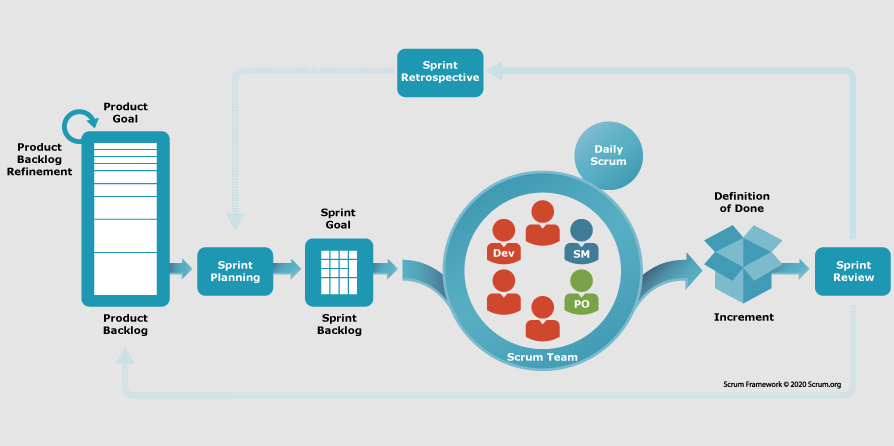
\includegraphics[width=\textwidth, height=4cm]{figures/scrum-overview.png}
	\caption{Scrum Overview}
\end{figure}


\newpage 

\section{Scrum Activities and Events}
\begin{itemize}
	\item \textbf{Sprint Planning.}  \hfill \vspace{0.2cm} \\
	Each sprint begins with a sprint planning meeting, where the team leader presents the top items on the product backlog to the team, and team members figure out how much work they can commit to during the coming sprint.
	
	\item \textbf{The Sprint.} \hfill \vspace{0.2cm} \\
	During each sprint, the team takes a small set of features from idea to fully implemented and tested functionality. At the end, these features are done and could potentially be released.
	
	\item \textbf{Daily Scrum.} \hfill \vspace{0.2cm} \\
	On each day of the sprint, all team members attend a daily scrum meeting. Daily scrums are a way for team members to synchronize their work and collaborate to move that work to done. The daily meetings last no more than 15 minutes and are intended to give the team a time to share what they worked on the prior day, will work on that day, and identify any impediments to progress.
	
	\item  \textbf{Sprint Review.}  \hfill \vspace{0.2cm} \\
	At the end of a sprint, the team conducts a sprint review during which the team demonstrates the new functionality to the stakeholder who wishes to provide feedback that could influence the next sprint. It's critical that the sprint review remains informal and doesn't become its own task, distracting from the work itself.
\end{itemize}

\section{Why Scrum?}
\begin{enumerate}
	\item \textbf{Responsive team:} 
	with scrum, our teams will be more responsive in their productivity, especially as changes and pivots are required. The scrum discipline requires frequent reviewing of progress, which often demands changes to prevent a project from failing.
	
	\item \textbf{More accurate planning:}
	by using Scrum, our plans will be less apt to fail. Why? Because our teams are constantly putting in the effort to keep them on track by shifting and changing as needed. And because of the way scrum is designed, our teams will constantly be reflecting how things are going and can make small or large adjustments to the plans, according to the winds of change. By adhering to scrum artifacts and events, our plans are far less likely to fail.
	
	\item \textbf{Everyone in sync:}
	when using scrum, a project’s stakeholders are always in sync. And because the scrum methodology prioritizes individuals and interactions over all else, keeping everyone involved in sync is actually built into the process.
	
	\item \textbf{Flexible priorities:}
	with scrum, it’s very easy to prioritize and re-prioritize as the project moves through the process. With this ability, our developer team become more flexible and our project becomes more agile. This also makes it possible to easily (and quickly) adjust short-term goals while still adhering to the overall strategy of the project.
	
	\item \textbf{More control:}
	finally, we will have more control over the entire project. That’s not to say we will be able to better control our staff. No. Instead, we have more control over the direction and flow of the development process. And when we have consistent input from developers and other stakeholders, it lends a level of cohesion to the process you wouldn’t otherwise have.
\end{enumerate}

\section{Main tasks of our project}
\begin{itemize}
    \item Design UI and UX
    \item Design database diagrams
    \item Implement the frontend
    \item Implement the backend
    \item Test and debug the project
    \item Writing the documentation
\end{itemize}

\newpage

\begin{figure}[h!]
	\centering
	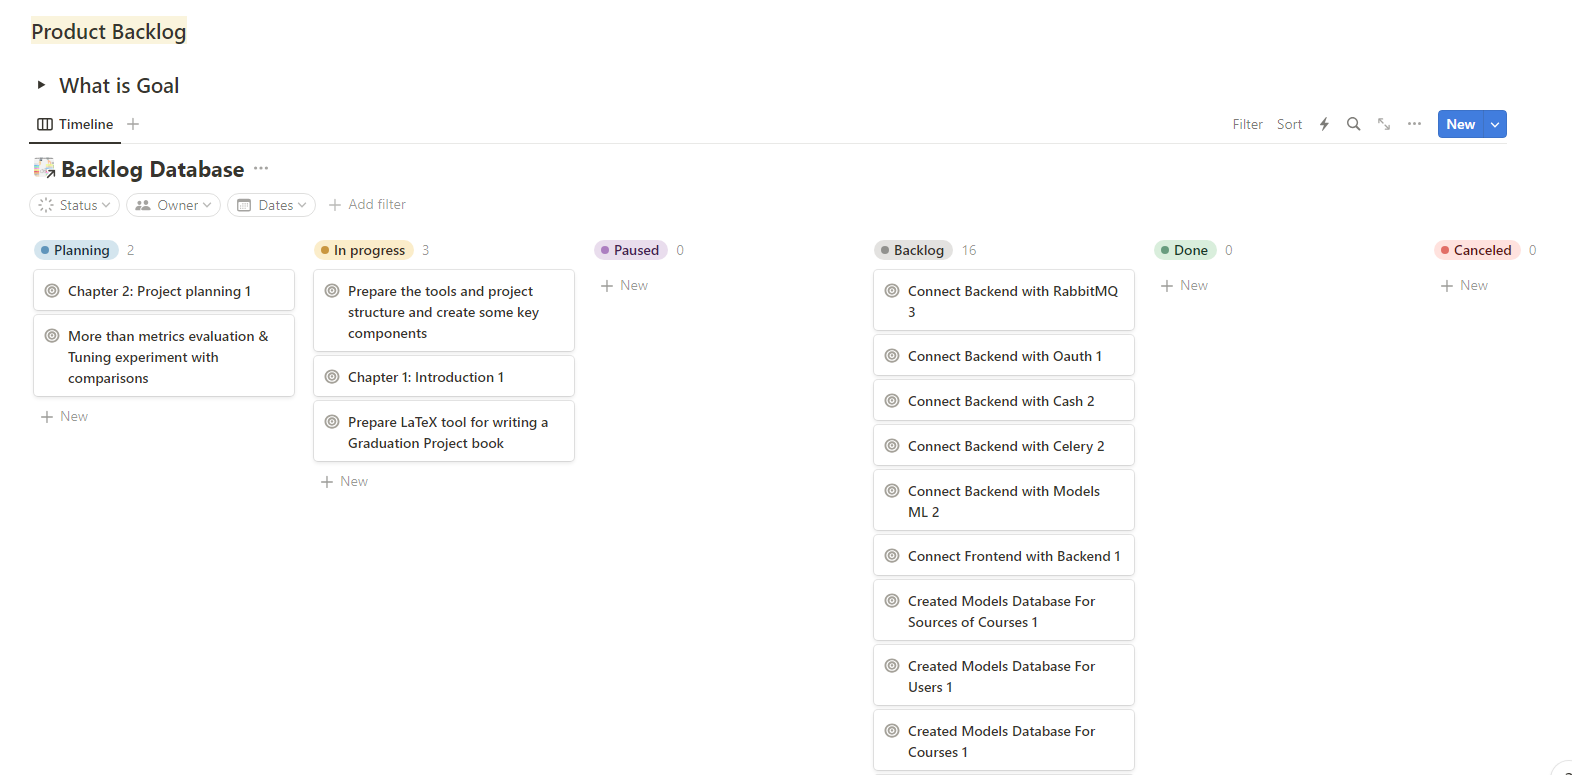
\includegraphics[width=0.95\textwidth]{figures/snapshot-of-backlog-database.png}
	\caption{Snapshot Of backlog}
\end{figure}

\begin{figure}[h!]
	\centering
	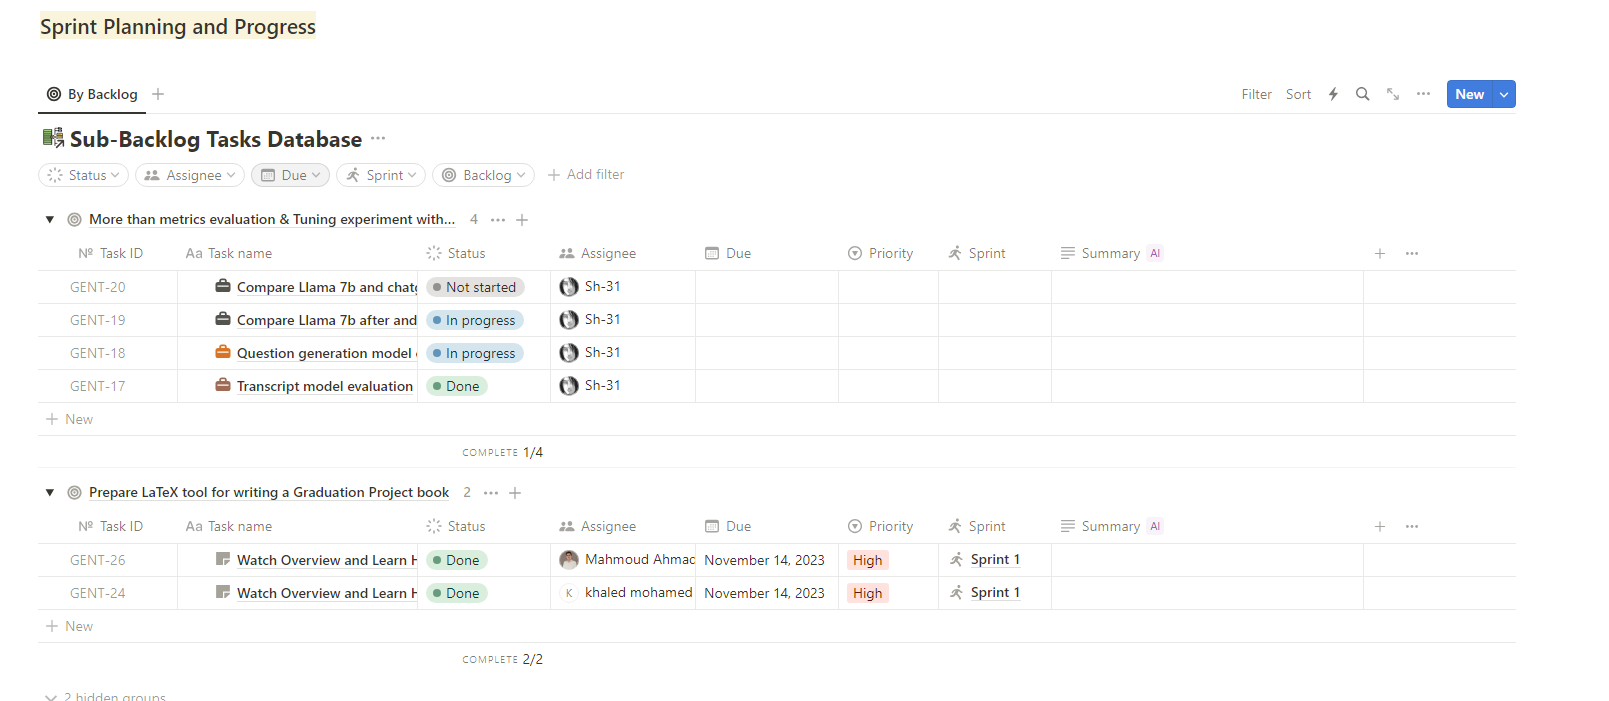
\includegraphics[width=0.95\textwidth]{figures/snapshot-of-sprint-planning.png}
	\caption{Snapshot Of sprint planning}
\end{figure}

\newpage 

\section{Risk Identification}
Project Risk Management includes the processes of conducting 
risk management planning, identification, analysis, response 
planning, and controlling risk on a project. The objectives 
of project risk management are to increase the likelihood and 
impact of positive events and decrease the likelihood and impact 
of negative events in the project. The key step in risk management
planning is project risk identification. Risk identification
identifies the risks that could have an impact on the project 
and lists their characteristics. However, as recommended, we should
avoid devoting too much time to risk identification.

\subsection{Technology Dependencies}
\textbf{Risk:} Dependencies on third-party technologies or frameworks may undergo updates or discontinuation, impacting the platform's functionality. \\
\textbf{Mitigation:} Regularly update and maintain dependencies, conduct thorough compatibility checks, and have contingency plans for potential disruptions.

\subsection{Data Security and Privacy}
\textbf{Risk:} Security breaches or data privacy issues could compromise user information and erode trust. \\
\textbf{Mitigation:} Implement robust security measures, adhere to data protection regulations, and conduct regular security audits to identify and address vulnerabilities.

\subsection{User Adoption}
\textbf{Risk:} Users may find the platform challenging to navigate, leading to low adoption rates. \\
\textbf{Mitigation:} Implement a user-friendly onboarding process, provide clear documentation, and offer responsive customer support to ensure users can easily navigate and utilize the platform.

\newpage 

\subsection{Scalability Challenges}
\textbf{Risk:} An unexpected surge in user traffic may lead to server overload, causing system slowdowns or crashes. \\
\textbf{Mitigation:} Utilize scalable cloud services, conduct load testing, and have a scalable infrastructure in place to accommodate a growing user base.

\subsection{Content Quality}
\textbf{Risk:} Inaccuracies or insufficient quality in course content may impact the effectiveness of the learning experience. \\
\textbf{Mitigation:} Establish a thorough content review process, actively seek user feedback on content quality, and iterate based on user input.

\subsection{Technological Obsolescence}
\textbf{Risk:} Rapid advancements in technology may render certain components of the platform obsolete. \\
\textbf{Mitigation:} Regularly update the technological stack, monitor emerging technologies, and plan for phased upgrades to avoid obsolescence.

\subsection{Adaptability to Learning Styles}
\textbf{Risk:} The platform may not fully cater to the diverse learning styles and preferences of users. \\
\textbf{Mitigation:} Gather user feedback on learning experiences, conduct usability testing with a diverse user base, and iterate the platform design to enhance adaptability.

\subsection{Integration with External Systems}
\textbf{Risk:} Challenges in integrating seamlessly with external platforms or tools may hinder collaboration opportunities. \\
\textbf{Mitigation:} Conduct thorough compatibility testing with external systems, establish robust APIs, and foster collaborations through ongoing communication with potential partners.

\newpage 

\subsection{Regulatory Compliance}
\textbf{Risk:} Changes in educational or data protection regulations may necessitate adjustments to the platform. \\
\textbf{Mitigation:} Stay informed about regulatory changes, conduct regular compliance checks, and adapt the platform accordingly to ensure alignment with current standards.

\subsection{User Technical Proficiency}
\textbf{Risk:} Users with limited technological skills may struggle to navigate and utilize the platform effectively. \\
\textbf{Mitigation:} Provide comprehensive user guides, tutorials, and responsive customer support to assist users with varying levels of technical proficiency.


